

\tikzset{every picture/.style={line width=0.75pt}} %set default line width to 0.75pt        

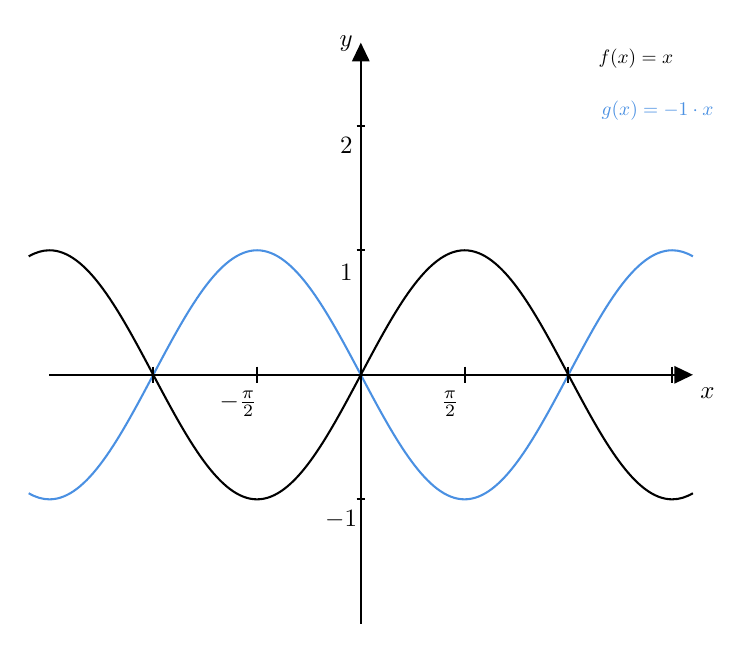
\begin{tikzpicture}[x=0.75pt,y=0.75pt,yscale=-1,xscale=1]
%uncomment if require: \path (0,328); %set diagram left start at 0, and has height of 328

%Shape: Wave [id:dp94416819522044] 
\draw   (180,122.94) .. controls (183.26,121.04) and (186.58,120) .. (190,120) .. controls (208.1,120) and (223.69,149.26) .. (240,180) .. controls (256.31,210.74) and (271.9,240) .. (290,240) .. controls (308.1,240) and (323.69,210.74) .. (340,180) .. controls (356.31,149.26) and (371.9,120) .. (390,120) .. controls (408.1,120) and (423.69,149.26) .. (440,180) .. controls (456.31,210.74) and (471.9,240) .. (490,240) .. controls (493.42,240) and (496.74,238.96) .. (500,237.06) ;
%Shape: Wave [id:dp05495114548578883] 
\draw  [color={rgb, 255:red, 74; green, 144; blue, 226 }  ,draw opacity=1 ] (180,237.06) .. controls (183.26,238.96) and (186.58,240) .. (190,240) .. controls (208.1,240) and (223.69,210.74) .. (240,180) .. controls (256.31,149.26) and (271.9,120) .. (290,120) .. controls (308.1,120) and (323.69,149.26) .. (340,180) .. controls (356.31,210.74) and (371.9,240) .. (390,240) .. controls (408.1,240) and (423.69,210.74) .. (440,180) .. controls (456.31,149.26) and (471.9,120) .. (490,120) .. controls (493.42,120) and (496.74,121.04) .. (500,122.94) ;
%Straight Lines [id:da13690129851328403] 
\draw    (190,180) -- (498,180) (240,176) -- (240,184)(290,176) -- (290,184)(340,176) -- (340,184)(390,176) -- (390,184)(440,176) -- (440,184)(490,176) -- (490,184) ;
\draw [shift={(500,180)}, rotate = 180] [fill={rgb, 255:red, 0; green, 0; blue, 0 }  ][line width=0.75]  [draw opacity=0] (8.93,-4.29) -- (0,0) -- (8.93,4.29) -- cycle    ;

%Straight Lines [id:da021329477973490496] 
\draw    (340,300) -- (340,22) (338,240) -- (342,240)(338,180) -- (342,180)(338,120) -- (342,120)(338,60) -- (342,60) ;
\draw [shift={(340,20)}, rotate = 450] [fill={rgb, 255:red, 0; green, 0; blue, 0 }  ][line width=0.75]  [draw opacity=0] (8.93,-4.29) -- (0,0) -- (8.93,4.29) -- cycle    ;


% Text Node
\draw (472.5,27.5) node [scale=0.7]  {$f( x) =\sen x$};
% Text Node
\draw (383,194) node [scale=0.9,color={rgb, 255:red, 0; green, 0; blue, 0 }  ,opacity=1 ]  {$\frac{\pi }{2}$};
% Text Node
\draw (281,194) node [scale=0.9,color={rgb, 255:red, 0; green, 0; blue, 0 }  ,opacity=1 ]  {$-\frac{\pi }{2}$};
% Text Node
\draw (333,130.5) node [scale=0.9]  {$1$};
% Text Node
\draw (330.5,249.5) node [scale=0.9]  {$-1$};
% Text Node
\draw (483,52.5) node [scale=0.7,color={rgb, 255:red, 74; green, 144; blue, 226 }  ,opacity=1 ]  {$g( x) =-1\cdot \sen x$};
% Text Node
\draw (507,189) node [scale=0.9]  {$x$};
% Text Node
\draw (333,20.5) node [scale=0.9]  {$y$};
% Text Node
\draw (333,69.5) node [scale=0.9]  {$2$};


\end{tikzpicture}
